% TerraScope Crop Health Monitor -- IEEE conference paper (IEEEtran).
% Compile: pdflatex terrascope-ieee && bibtex terrascope-ieee && pdflatex terrascope-ieee && pdflatex terrascope-ieee
\documentclass[conference]{IEEEtran}
\IEEEoverridecommandlockouts

\usepackage{cite}
\usepackage{amsmath,amssymb,amsfonts}
\usepackage{graphicx}
\usepackage{textcomp}
\usepackage{xcolor}
\usepackage{booktabs}
\usepackage{multirow}
\usepackage{algorithm}
\usepackage{algpseudocode}
\usepackage{tikz}
\usetikzlibrary{positioning,arrows.meta,fit}
\usepackage{url}
\usepackage[hidelinks]{hyperref}

\graphicspath{{figures/}}
\newcommand{\NDVI}{\mathrm{NDVI}}

\begin{document}

\title{TerraScope: An Evidence-First, Provenance-Aware Platform for Field-Level Crop Health Monitoring with Sentinel-2 Imagery}

\author{
\IEEEauthorblockN{Tushar Singh\textsuperscript{*}}
\IEEEauthorblockA{\textit{School of Computer Science and Engineering}\\
\textit{IILM University}\\
Greater Noida, India\\
tushar.singh.cs28@iilm.edu}
\and
\IEEEauthorblockN{Anurodh Singh}
\IEEEauthorblockA{\textit{School of Computer Science and Engineering}\\
\textit{IILM University}\\
Greater Noida, India\\
anurodh.singh.cs28@iilm.edu}
\and
\IEEEauthorblockN{Vansh Thakur}
\IEEEauthorblockA{\textit{School of Computer Science and Engineering}\\
\textit{IILM University}\\
Greater Noida, India\\
vansh.thakur.cs28@iilm.edu}
\and
\IEEEauthorblockN{Sahil Sharma}
\IEEEauthorblockA{\textit{School of Computer Science and Engineering}\\
\textit{IILM University}\\
Greater Noida, India\\
sahil.sharma.cs28@iilm.edu}
\thanks{\textsuperscript{*}Corresponding author.}}

\maketitle

\begin{abstract}
Satellite crop-monitoring dashboards commonly turn vegetation indices into a single health score, even when the image is cloudy, stale, or covers only part of the field. We present TerraScope, an open platform for field-level monitoring from Sentinel-2 imagery that treats the quality of its evidence as an output. It masks invalid pixels with the scene classification layer, accepts a measurement only if the valid share of the whole field boundary reaches a minimum coverage (default 70\%), and binds every observation to its scene, boundary revision, calculation method and provenance. A five-state assessment keeps ``needs inspection'' separate from ``image too old'' and ``not enough data''. We evaluate the platform in three layers. Controlled tests on the production raster endpoint recover masked field means to within $5\times10^{-5}$ and show the coverage gate switching at the specified cloud fraction. An audit on 3\,725 real fields of the Telangana Crop Health Challenge supports the measurement layer: an independent cloud score disagrees strongly with only 0.3\% of accepted images, and removing edge pixels changes the decline decision for at most 1.0\% of image pairs. The same audit shows that the default decision rule has no discriminative power against the survey labels (alert rate 79.9\% on problem fields versus 78.6\% on healthy fields; AUC 0.498), fires on 12.2\% of healthy mid-season image pairs, and receives only partial independent support from recorded harvest dates and none from rainfall. We conclude that evidence-first design is necessary but not sufficient: dated, expert-verified labels are required before any stress-detection claim.
\end{abstract}

\begin{IEEEkeywords}
precision agriculture, Sentinel-2, NDVI, remote sensing, data provenance, cloud masking, Google Earth Engine, crop health monitoring, label leakage, smallholder farming
\end{IEEEkeywords}

%=====================================================================
\section{Introduction}
%=====================================================================
Most of the world's farms are small: farms under two hectares make up the large majority of holdings worldwide~\cite{lowder2016}, and in India they are often managed without agronomic advisory support. Free multispectral imagery from the Sentinel-2 constellation~\cite{drusch2012}, at 10--20\,m resolution and with a revisit time of about five days, makes field-level monitoring technically possible for such farms. Vegetation indices such as the normalized difference vegetation index (NDVI)~\cite{rouse1974} are well established proxies for canopy vigour~\cite{mulla2013,weiss2020}.

Turning an index into advice, however, involves decisions that many consumer dashboards hide. A parcel may be 60\% cloud-covered on the most recent pass; the newest usable image may be three weeks old; a farmer may have redrawn the boundary since the last measurement. An index value can also fall because of harvest, senescence or irrigation rather than disease. When a dashboard reports a single ``health score'' regardless of these conditions, the absence of evidence is shown to the user as evidence of health.

TerraScope (Crop Health Monitor) is designed around the opposite principle: \emph{a measurement is only as useful as the evidence behind it, and the absence of usable evidence must be shown as such}. This paper makes the following contributions:
\begin{enumerate}
  \item An \textbf{evidence-first assessment model} that binds every vegetation measurement to its scene, field-boundary revision, calculation version and provenance, and that reports five explicit attention states instead of a universal health score (Section~\ref{sec:evidence}).
  \item A \textbf{boundary-normalized quality gate} for Sentinel-2 L2A data that uses the whole field as the coverage denominator, refuses to guess reflectance scaling, and rejects scenes below a configurable coverage and pixel threshold (Section~\ref{sec:engine}).
  \item A complete, open \textbf{system implementation} with a bilingual interface, PostGIS data model, a durable lease-based job queue, Google Earth Engine integration, and six public reference datasets attached with field-level provenance (Section~\ref{sec:arch}).
  \item A \textbf{controlled evaluation of the production raster endpoint} that quantifies measurement accuracy, quality-gate behaviour, and the sensitivity limits of the default change-detection rules (Section~\ref{sec:results}).
  \item A \textbf{real-imagery audit} on 3\,725 labelled Telangana fields: false-reassurance, false-trigger and injected-stress rates of the shipped decision rule; an independent validation of the cloud mask with Cloud Score+; edge-pixel and field-size breakdowns; and independent checks from recorded harvest dates and rainfall (Sections~\ref{sec:method} and~\ref{sec:results}). The audit reports a negative result for the decision rule.
  \item A \textbf{leakage audit} of public crop-health benchmarks, with honest leakage-controlled baselines.
\end{enumerate}

%=====================================================================
\section{Related Work}
%=====================================================================
\subsection{Spectral indices and Sentinel-2 processing}
NDVI~\cite{rouse1974} contrasts near-infrared (NIR) and red reflectance. SAVI~\cite{huete1988} adds a soil-brightness correction, EVI~\cite{huete2002} reduces atmospheric and canopy-saturation effects using the blue band, red-edge indices (NDRE) track chlorophyll content~\cite{gitelson1994}, and SWIR-based moisture indices (NDMI/NDWI) respond to canopy water~\cite{gao1996}. Sentinel-2 Level-2A products are generated by Sen2Cor~\cite{mainknorn2017}, which also produces a scene classification layer (SCL) that labels cloud, cloud shadow, cirrus, snow and defective pixels. Google Earth Engine~\cite{gorelick2017} and STAC-based catalogues~\cite{stac} make these products available without bulk downloads.

\subsection{Crop monitoring systems and reference data}
Reviews of agricultural remote sensing~\cite{mulla2013,weiss2020} identify a persistent gap between index products and validated, field-scale decision support, mainly because of the scarcity of ground truth. Global reference products, including ESA WorldCover~\cite{zanaga2022}, ESA WorldCereal~\cite{vantricht2023}, CHIRPS rainfall~\cite{funk2015}, SoilGrids~\cite{poggio2021} and NASA POWER meteorology~\cite{nasapower}, provide context but not field-level, current-season truth. CropHarvest~\cite{tseng2021} provides harmonized crop/non-crop and crop-type labels with remote-sensing features for benchmarking.

\subsection{Image-based disease recognition and evaluation pitfalls}
Deep convolutional networks reach very high accuracy on the PlantVillage leaf images~\cite{hughes2015,mohanty2016,ferentinos2018}, but performance falls sharply on field photographs with complex backgrounds~\cite{mohanty2016,barbedo2018}. More generally, random cross-validation overstates performance for spatially structured data~\cite{roberts2017,ploton2020}, and target information leaking into features produces optimistic results~\cite{kaufman2012}. TerraScope's design and evaluation take these lessons as constraints: spatial and source hold-outs, duplicate checks, and an explicit refusal to call proxy labels ground truth. Data handling follows the provenance and FAIR principles~\cite{provdm2013,wilkinson2016}.

\subsection{Existing monitoring tools and cloud-mask validation}\label{sec:tools}
Table~\ref{tab:tools} compares TerraScope with three widely used, publicly documented tools that show Sentinel-2 vegetation indices for user-selected fields or areas. The comparison is limited to what the vendors and agencies state in their public documentation as of November 2026; we did not run these tools, and ``not documented'' does not mean ``absent''. The point it supports is narrow: the tools document cloud handling at the scene level, or as hiding or skipping cloudy images, whereas TerraScope attaches a field-level validity figure and an explicit unknown state to every measurement, and Section~\ref{sec:results} tests that behaviour.

\begin{table}[t]
\caption{Documented cloud handling and change alerts in related tools (public documentation, Nov. 2026)}
\label{tab:tools}
\centering
\resizebox{\columnwidth}{!}{%
\begin{tabular}{@{}p{1.6cm}p{2.0cm}p{3.2cm}p{2.5cm}@{}}
\toprule
Tool & Imagery & Cloud handling (documented) & Change alerts \\
\midrule
OneSoil~\cite{onesoilhelp} & Sentinel-2 & Detects cloud, shadow and snow; NDVI computed only where clear; updates every 3--5 days & Not documented in the pages consulted \\
EOSDA Crop Monitoring~\cite{eosdadocs} & Sentinel-2 (10\,m); optional PlanetScope & User-adjustable cloud and shadow threshold; images above 50\% cloud hidden by default & Alerts on abnormal negative NDVI change (vendor description) \\
Copernicus Browser~\cite{cdsebrowser} & Sentinel-2 L2A & Cloud filter applied to the whole scene (default 30\%), not to the field & None (visualization only) \\
\textbf{TerraScope} & Sentinel-2 L2A (Earth Engine) & Per-pixel SCL mask; whole-field coverage gate ($\ge$70\%); stale or thin evidence shown as ``unknown'' & Decline rule on accepted, comparable pairs only (Alg.~\ref{alg:assess}) \\
\bottomrule
\end{tabular}}
\end{table}

Cloud masks themselves have been validated against reference masks. Sen2Cor's scene classification, which TerraScope uses, reached about 84\% overall accuracy against reference masks, below MAJA and Fmask at about 90--91\%~\cite{baetens2019}, and an international intercomparison found good agreement on thick cloud but not on thin or semi-transparent cloud~\cite{skakun2022}. Those studies score pixels over whole scenes. They do not report how many \emph{field-level} decisions change, which is what matters here and what Section~\ref{sec:results} measures, using Cloud Score+~\cite{pasquarella2023} as an independent reference.

%=====================================================================
\section{System Architecture}\label{sec:arch}
%=====================================================================
\begin{figure}[t]
\centering
\resizebox{\columnwidth}{!}{%
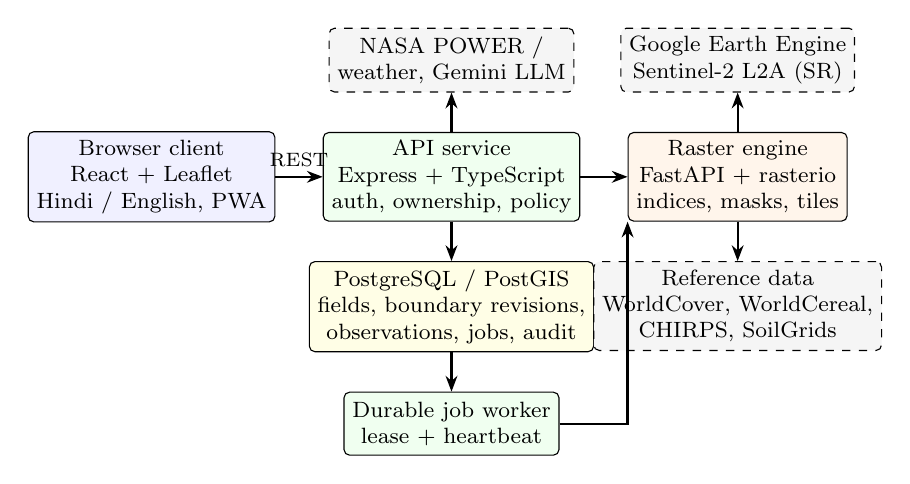
\begin{tikzpicture}[
  node distance=5mm and 6mm,
  box/.style={draw, rounded corners=2pt, align=center, font=\footnotesize, minimum height=8mm, inner sep=3pt, fill=white},
  ext/.style={box, dashed, fill=gray!8},
  arr/.style={-{Stealth[length=2mm]}, thick}]
  \node[box, fill=blue!6]   (ui)  {Browser client\\React + Leaflet\\Hindi / English, PWA};
  \node[box, fill=green!6, right=of ui]  (api) {API service\\Express + TypeScript\\auth, ownership, policy};
  \node[box, fill=orange!8, right=of api] (eng) {Raster engine\\FastAPI + rasterio\\indices, masks, tiles};
  \node[box, fill=yellow!10, below=of api] (db) {PostgreSQL / PostGIS\\fields, boundary revisions,\\observations, jobs, audit};
  \node[box, fill=green!6, below=of db] (wk) {Durable job worker\\lease + heartbeat};
  \node[ext, above=of eng] (gee) {Google Earth Engine\\Sentinel-2 L2A (SR)};
  \node[ext, below=of eng] (ref) {Reference data\\WorldCover, WorldCereal,\\CHIRPS, SoilGrids};
  \node[ext, above=of api] (wx) {NASA POWER /\\weather, Gemini LLM};
  \draw[arr] (ui) -- node[above, font=\scriptsize]{REST} (api);
  \draw[arr] (api) -- (eng);
  \draw[arr] (api) -- (db);
  \draw[arr] (db) -- (wk);
  \draw[arr] (wk.east) -| (eng.south west);
  \draw[arr] (eng) -- (gee);
  \draw[arr] (eng) -- (ref);
  \draw[arr] (api) -- (wx);
\end{tikzpicture}}
\caption{TerraScope architecture. Solid boxes are TerraScope components; dashed boxes are external providers. Only the API talks to the database; the raster engine is stateless.}
\label{fig:arch}
\end{figure}

Fig.~\ref{fig:arch} shows the three-tier architecture. The \textbf{client} is a React~19/Vite single-page application with Leaflet and OpenStreetMap for field drawing, boundary editing and overlay display; no map API key is needed. The interface is bilingual (Hindi/English) with a bundled Devanagari font, supports hectare/acre units, and adapts from 320\,px phones to desktops. The \textbf{API} (Express~5, TypeScript) handles accounts, per-field ownership checks, request limits, evidence policy and exports. The \textbf{raster engine} (FastAPI, rasterio, Shapely, Earth Engine Python API) is stateless: it receives a boundary and asset references and returns statistics, overlays or map tiles. State is kept in \textbf{PostgreSQL~18 with PostGIS~3.6}, managed by 18 additive migrations.

\subsection{Provenance-preserving data model}
A field has a polygon boundary and an integer \emph{boundary version}. Editing a boundary archives the old geometry, increments the version, invalidates summaries and fails any queued job created for the old version. Each observation stores the scene identifier, acquisition timestamp, source (Earth Engine or Earth Search), \texttt{calculation\_version}, valid-pixel count, valid coverage, an \texttt{accepted} flag with a quality reason, and one of five provenance classes: \texttt{measured\_imagery}, \texttt{user\_reported}, \texttt{public\_boundary}, \texttt{demo} and \texttt{legacy\_unverified}. Only accepted \texttt{measured\_imagery} on the current boundary version can influence an assessment, so legacy or synthetic values cannot be silently promoted.

Fig.~\ref{fig:record} shows one stored observation from the deployed database (identifiers replaced), and Fig.~\ref{fig:ui} shows how the same data reach the user: the ``what changed'' banner and the NDVI series with the colour bands used everywhere in the interface, followed by the best NDVI of each calendar month, where months without a clear picture stay empty.

\begin{figure}[t]
\centering
\scriptsize
\begin{verbatim}
{ "field_id": "<uuid>", "boundary_version": 1,
  "observed_on": "2026-11-18",
  "scene_id": "gee-20261118T051109_..._T44RNQ",
  "tile_id": "44RNQ",
  "source": "Copernicus Sentinel-2 via GEE",
  "provenance": "measured_imagery",
  "calculation_version":
      "gee-sentinel-reflectance-scl-v1",
  "accepted": true, "quality_reason": null,
  "valid_pixel_count": 758,
  "valid_coverage_percent": 100.00,
  "ndvi_value": 0.453, "ndvi_median": 0.4318,
  "ndvi_min": 0.2611, "ndvi_max": 0.8125,
  "ndre_value": 0.291, "ndmi_value": 0.063,
  "ndvi_classes": { "bare": 0, "low": 32.5,
      "moderate": 55.9, "high": 11.7 } }
\end{verbatim}
\caption{A stored observation (abridged; identifiers replaced). Scene, tile, boundary revision, calculation version, provenance, coverage and the acceptance decision with its reason are stored with every value.}
\label{fig:record}
\end{figure}

\begin{figure}[t]
\centering
\includegraphics[width=0.78\columnwidth]{fig_ui_analysis.png}
\caption{The ``Changes over time'' screen, rendered from real stored readings of a rice field (English interface; a Hindi interface is available). Top: the latest-change banner and the NDVI series with the colour bands. Bottom: best NDVI of each month; months without a clear picture are left empty.}
\label{fig:ui}
\end{figure}

\subsection{Durable processing jobs}
Image checks run as PostgreSQL-backed jobs rather than in the request cycle. A unique partial index on (\textit{field}, \textit{kind}) for active states deduplicates repeated requests. Workers claim jobs with \texttt{SELECT \dots{} FOR UPDATE SKIP LOCKED}, write a heartbeat every 20\,s under a random lease token, and a recovery pass re-queues jobs whose heartbeat is older than 6\,min until their attempt budget is exhausted. A job whose field boundary has changed is failed rather than allowed to attach results to the wrong geometry. Closing the browser therefore does not cancel processing, and a crashed worker cannot leave a job stuck.

\subsection{Reference datasets}
Six public sources can be attached per field, each stored as a boundary-versioned run with source, licence, retrieval time and coverage: ESA WorldCover 2021 (land-cover shares)~\cite{zanaga2022}, ESA WorldCereal 2021 temporary-crop maps via Earth Engine~\cite{vantricht2023}, CHIRPS~v3 daily rainfall~\cite{funk2015}, SoilGrids~2.0 surface properties with uncertainty quantiles~\cite{poggio2021}, NASA POWER daily weather~\cite{nasapower}, and permission-reviewed FAO crop-calendar rows. Raster downloads use bounded HTTP range requests on the intersecting tile only, and the system refuses a global-raster fallback. These sources are shown as historical or modeled \emph{context}; they are never used as the current crop identity or as soil-test results.

\subsection{Ground-truth collection with consent}
Farmers can record photo-backed scouting notes with a category, growth stage and severity. The API always stores them as \texttt{owner\_reported}/\texttt{unverified}, whatever the client submits. Per note, an owner may consent to a research field visit; consent events are append-only. A reviewer role, granted only by a database operator, unlocks a queue that shows consented field locations and dates but hides the farmer's photos, notes and labels to reduce anchoring bias. Reviewers submit independent labels with a field-visit attestation into a separate, append-only table. A pure TypeScript evaluator computes confusion-matrix metrics from \emph{expert-verified} records only, returns \texttt{null} rather than 0 for undefined denominators, and asserts that no field appears in both training and evaluation sets.

\subsection{Assistant and leaf-photo research tools}
An optional Gemini-based assistant receives recent field records with instructions to describe farmer reports as reports, not diagnoses. Leaf-photo classifiers (Section~\ref{sec:ml}) are isolated research endpoints that accept only signature-verified JPEG/PNG/WebP images under 5\,MB and 20\,MP, process uploads in memory, and return explicitly uncalibrated class scores.

%=====================================================================
\section{Field-Level Index Computation}\label{sec:engine}
%=====================================================================
\subsection{Reflectance handling and masking}
For a boundary polygon $P$ (WGS84), the engine reprojects $P$ into the CRS of the red band and builds a reference grid $G$ that covers the entire bounding box of $P$, even where it extends beyond the scene footprint. Every band is warped onto $G$ (bilinear for reflectance, nearest-neighbour for the categorical SCL) and converted to surface reflectance $\rho = s\cdot DN + o$ using the STAC \texttt{raster:bands} scale $s$ and offset $o$. If an integer band arrives without trustworthy scale and offset metadata, the engine raises an error rather than guessing. A pixel $p$ is \emph{valid} if
\begin{equation}
p \in P,\quad \mathrm{SCL}(p) \notin \mathcal{I},\quad \rho_{\mathrm{red}},\rho_{\mathrm{NIR}} \ge 0,\quad |\rho_{\mathrm{NIR}}+\rho_{\mathrm{red}}| > 10^{-12},
\end{equation}
where $\mathcal{I}=\{0,1,2,3,8,9,10,11\}$ excludes no-data, saturated/defective, dark-area, cloud-shadow, medium- and high-probability cloud, thin-cirrus and snow pixels~\cite{mainknorn2017}. A missing SCL band is an error, not a reason to skip masking.

\subsection{Indices}
Over the valid set $V$ the engine reports
\begin{align}
\NDVI &= \frac{\rho_{\mathrm{NIR}}-\rho_{\mathrm{red}}}{\rho_{\mathrm{NIR}}+\rho_{\mathrm{red}}}, \quad
\mathrm{NDRE} = \frac{\rho_{\mathrm{NIR}}-\rho_{\mathrm{RE1}}}{\rho_{\mathrm{NIR}}+\rho_{\mathrm{RE1}}},\\
\mathrm{NDMI} &= \frac{\rho_{\mathrm{NIR}}-\rho_{\mathrm{SWIR1}}}{\rho_{\mathrm{NIR}}+\rho_{\mathrm{SWIR1}}}, \quad
\mathrm{SAVI} = \frac{1.5(\rho_{\mathrm{NIR}}-\rho_{\mathrm{red}})}{\rho_{\mathrm{NIR}}+\rho_{\mathrm{red}}+0.5},\\
\mathrm{EVI} &= \frac{2.5(\rho_{\mathrm{NIR}}-\rho_{\mathrm{red}})}{\rho_{\mathrm{NIR}}+6\rho_{\mathrm{red}}-7.5\rho_{\mathrm{blue}}+1},
\end{align}
together with the mean, median, minimum, maximum and standard deviation of NDVI. Sentinel-2 bands B4, B8, B5, B11 and B2 supply red, NIR, RE1, SWIR1 and blue respectively.

\subsection{Coverage and acceptance}
The quality denominator is the number of grid cells inside the \emph{whole} boundary, so a field half outside a scene cannot appear fully observed:
\begin{equation}
C = 100\cdot\frac{|V|}{|\{p\in G : p\in P\}|}.
\end{equation}
An observation is accepted if $C \ge C_{\min}$ and $|V|\ge N_{\min}$, with defaults $C_{\min}=70\%$ and $N_{\min}=10$. Candidate scenes from the last 90 days (in the Earth Engine path, pre-filtered to \texttt{CLOUDY\_PIXEL\_PERCENTAGE}~$<40$) are processed newest first, up to six attempts. If no candidate is accepted, the previous evidence stays in place; it is not overwritten with a poorer measurement.

\subsection{Within-scene anomaly zones}
To guide scouting, pixels with $\NDVI(p) < \mu_V - 1.5\,\sigma_V$ are vectorized into ``inspection zones'' and reported as an affected-area percentage. These zones are a visit aid, not a stress classification; Section~\ref{sec:results} quantifies their behaviour.

%=====================================================================
\section{Evidence-First Assessment}\label{sec:evidence}
%=====================================================================
\begin{algorithm}[t]
\caption{Field assessment from accepted evidence}
\label{alg:assess}
\begin{algorithmic}[1]
\Require latest observation $L$ with valid coverage $C_L$ (\%), valid-pixel count $N_L$, provenance $L.\mathit{prov}$ and NDVI $\NDVI_L$; previous observation $R$ of the same field with NDVI $\NDVI_R$; policy $(C_{\min},N_{\min},F,\delta)$: minimum coverage $C_{\min}$ (\%), minimum valid pixels $N_{\min}$, freshness limit $F$ (days) and decline threshold $\delta$
\If{$L$ is none} \Return \textsc{AwaitingAnalysis} \EndIf
\State $a \gets$ age of $L$ in days (today minus acquisition date)
\If{$\neg L.\mathit{accepted}$ \textbf{or} $L.\mathit{prov}\neq\texttt{measured\_imagery}$ \textbf{or} $C_L<C_{\min}$ \textbf{or} $N_L<N_{\min}$}
  \State \Return \textsc{NotEnoughData}
\EndIf
\State $\Delta \gets$ none
\If{$R$ is accepted, measured, on the same boundary, calculation version and tile, earlier than $L$ and at most 30\,days older}
  \State $\Delta \gets \NDVI_L - \NDVI_R$
\EndIf
\If{$a > F$} \Return \textsc{ImageTooOld} \EndIf
\If{$\Delta \neq$ none \textbf{and} $\Delta \le -\delta$} \Return \textsc{NeedsInspection} \EndIf
\If{$\Delta =$ none} \Return \textsc{NotEnoughData} \EndIf
\State \Return \textsc{NoUnusualChange}
\end{algorithmic}
\end{algorithm}

Algorithm~\ref{alg:assess} gives the assessment rule, with defaults freshness $F=14$\,days and decline threshold $\delta=0.10$. Three properties matter. First, \emph{staleness takes priority over change}: an old image yields ``image too old; current crop condition is unknown'' even if it showed no decline. Second, a single usable image never produces a reassuring state, because change requires a comparable earlier image on the same boundary version and calculation version. Third, ``no unusual change'' is worded as ``this does not rule out crop problems'', and ``needs inspection'' lists harvest, maturity and bare soil as alternative explanations. Every state maps to one next action (find a newer image, plan a field visit, continue monitoring), which the bilingual dashboard shows first.

Multi-date trends are described with an ordinary least-squares slope over \emph{elapsed days}, not observation index. Same-day duplicates are averaged so that adjacent tiles do not count twice, and at least two distinct dates are required. The engine does not predict crop stage or future NDVI. An experimental 0--100 vegetation score ($0.75$ greenness $+\,0.25$ moisture) is shown only under advanced details and never affects acceptance.

%=====================================================================
\section{Experimental Methodology}\label{sec:method}
%=====================================================================
We evaluate TerraScope in three layers: (i) whether the engine measures what it claims under controlled conditions (E1, E2); (ii) how the shipped decision rules behave on real imagery, how reliable the cloud mask and the field geometry are, and whether independent evidence supports the change rule (E5--E7); and (iii) how public benchmarks behave under leakage-aware protocols (E3, E4). We do not claim agronomic accuracy for TerraScope's assessments, because no independently verified, dated field-health labels exist for the study region. The only labels available are season-level survey categories, which E5 uses with that limitation stated; E6 and E7 do not use the health labels at all.

\subsection{E1: Measurement accuracy and the coverage gate}
We drive the production \texttt{/calculate-indices} endpoint of the FastAPI engine (the same code path used for STAC assets) with synthetic GeoTIFFs on a $120\times120$ grid of $10^{-4}$\,degree ($\approx$11\,m) pixels. A square field covers 10\,000 pixels. Red reflectance is fixed at 0.08 and NIR is set so that per-pixel NDVI follows $\mathcal{N}(0.62, 0.06^2)$ exactly. Spatially clustered clouds, made by thresholding box-filtered Gaussian noise, are written into the SCL band (class~9) to cover 0--100\% of the field in steps of 5\%, with 10 random repetitions per level (210 runs). We record valid coverage, acceptance under the default policy, and absolute error against the true mean of clear pixels and of the whole field.

\subsection{E2: Sensitivity of the change rules}
For two dates, a base NDVI field $\mathcal{N}(0.70,0.05^2)$ is perturbed by independent noise $\mathcal{N}(0,0.02^2)$; on the second date a randomly placed square patch covering $f\in[0,0.6]$ of the field is reduced by 0.30 NDVI, a strong localized stress. Each of 13 levels is repeated 10 times (130 scene pairs, 260 endpoint calls). We measure the field-mean change $\Delta$, the share of pairs flagged by Algorithm~\ref{alg:assess} ($\Delta\le-0.10$), and the affected area returned by the $1.5\sigma$ zone rule.

\subsection{E3: Leakage-controlled learning baselines}\label{sec:ml}
\textit{CropHarvest crop/non-crop.} From 87\,464 checksum-verified CropHarvest~v14 samples~\cite{tseng2021} (216 features), 3\,143 duplicate-feature samples are removed. Four entire source datasets (\texttt{china-crop}, \texttt{kenya}, \texttt{lem-brazil}, \texttt{togo-eval}) are held out for testing, giving 79\,220 training and 5\,101 test samples. Cross-split location/date overlap is excluded, and no tuning uses the test set. A class-balanced random forest (100 trees, depth 12, seed 42) is trained.

\textit{Maize leaf disease.} A MobileNetV2~\cite{sandler2018} with a frozen ImageNet-pretrained backbone and a new four-class head (gray leaf spot, common rust, northern leaf blight, healthy) is trained on PlantVillage maize images~\cite{hughes2015} for 5 epochs (Adam, learning rate $10^{-3}$, batch 16, 224\,px, horizontal-flip augmentation). The split is 2\,599 training and 459 validation images, and evaluation uses the 794-image official test split.

\textit{Tabular crop-health baseline.} A previously committed baseline on a 212\,019-row tabular dataset (14 agronomic, weather and soil features, binary label) is audited against the majority-class rate.

\textit{Field-photo potato dataset.} The PLDD-UP dataset~\cite{plddup2026} (15\,519 field photographs from Uttar Pradesh: 4\,600 healthy, 4\,803 early blight, 6\,116 late blight) is inventoried with SHA-256 exact-duplicate and 64-bit difference-hash near-duplicate grouping, and groups are kept within one split. No trained-model result is reported for it, because training had not completed at the time of writing.

\subsection{E4: Live acquisition case and software verification}
We report a live public-boundary verification run and repository test results. All experiment scripts and raw outputs are in the project repository under \texttt{docs/paper/experiments}.

\subsection{Real-imagery data for E5--E7}\label{sec:realdata}
We use the Telangana Crop Health Challenge~\cite{telangana2024} (licence CC BY-SA 4.0). It provides field polygons for 3\,725 fields of at least 0.3\,ha (median 0.58\,ha, i.e.\ 30--282 Sentinel-2 pixels) in 14 districts, seven crops (cotton, maize, Bengal gram, groundnut, paddy, chillies, red gram) and the 2022--2024 seasons. Each field has one survey category per season (Healthy 3\,057, Pests 251, Stressed 211, Diseased 206), recorded sowing and harvest dates, and an irrigation source. The categories carry no date and are not expert field visits matched to image dates. For every field we obtained all Sentinel-2 L2A images (\texttt{COPERNICUS/S2\_SR\_HARMONIZED}) from 35\,days before sowing to 2\,days after the recorded harvest through Earth Engine, with the same reflectance scaling, SCL classes and NDVI formula as the production engine, which gave 391\,370 field-image rows. As in the application, each field uses one primary tile. The scripts and aggregate outputs are in the repository; the raw data are not redistributed.

\subsection{E5: Real-imagery audit of the shipped decision rule}
We replay the application's own code (Algorithm~\ref{alg:assess} and the visit decision of Section~\ref{sec:evidence}) on every accepted image between the recorded sowing and harvest dates, with the freshness age set to zero so that staleness cannot dominate. A field counts as \emph{alerted} if the replay says ``visit'' at least once in the season. Because labels are season-level, we report: (a) the alert rate in problem fields (Pests, Diseased, Stressed) and in healthy fields, and the area under the ROC curve (AUC) of the per-field share of alerting assessments, with a 95\% bootstrap interval; (b) \emph{false reassurance}, defined as a problem-labelled field that never alerted, together with the share of ``all clear'' decisions that rest on thin evidence (either image below 85\% coverage or below 30 valid pixels); (c) the \emph{false-trigger rate on stable conditions}, defined as the share of comparable image pairs with a change $\le-0.10$ among healthy-labelled fields whose recorded season is plausible (60--240\,days), restricted to the middle of the season (40--80\% of its length), where large genuine declines are least expected; and (d) \emph{injected stress}: to each of those real pairs we subtract $0.30f$ from the change, which is the field-mean effect of a localized drop of 0.30 over a share $f$ of the field (as in E2), so the response curve includes the real noise, cloud edges and phenology that E2 omits. Confidence intervals are Wilson intervals unless stated.

\subsection{E6: Cloud-mask validation, edge pixels and field size}
We draw a size-stratified random sample of 584 of the fields (120 per size class; 104 in the largest) and, through Earth Engine, summarize every Sentinel-2 image in the crop season (59\,121 field-image rows; 31\,104 on the primary tile). Per image we record the share of the field kept by the application's SCL mask, the share that Cloud Score+~\cite{pasquarella2023} calls clear (\texttt{cs\_cdf} $\ge0.6$; 0.5 and 0.65 as sensitivity), and the field-mean NDVI under the SCL mask and under both masks. Cloud Score+ is an independent, learned quality score; it is not ground truth, so we report disagreement, not error. We call an accepted image \emph{weakly unclear} if the reference calls at least 30\% of the field unclear and \emph{strongly unclear} if its mean score is below 0.30, which is much closer to real cloud or shadow. For edge pixels we recompute the SCL-masked NDVI over the polygon shrunk by 10\,m (one pixel) and compare it with the full polygon on the same images and gate, in terms of the pixel share removed, the NDVI shift, and the share of comparable pairs whose decline decision changes. All quantities are broken down by field area (0.3--0.4, 0.4--0.6, 0.6--1, 1--2 and $\ge2$\,ha).

\subsection{E7: Independent evidence from harvest dates and rainfall}
These checks do not use the health labels. (a)~\emph{Harvest dates.} For fields with a plausible season length (60--240\,days; 2\,522 fields) we align NDVI to the recorded harvest date, normalizing each field by its own season peak, and measure how often the decline rule fires as a function of days before harvest. If the dates are real, NDVI should peak well before them and decline events should concentrate in the last weeks. No images after harvest are in the extract, so a before/after comparison is not possible. (b)~\emph{Rainfall.} We join NASA POWER district rainfall~\cite{nasapower} to every comparable image pair in the growing stage (15--85\% of the season, gap 5--30\,days). In rainfed fields a dry spell should depress NDVI, whereas in irrigated fields it should not. We therefore compare the decline rate in the driest and wettest tercile of rainfall per day and the Spearman correlation between rainfall and NDVI change, separately for rainfed and irrigated fields and for the Kharif (monsoon) and Rabi seasons, with field-clustered bootstrap intervals. The thresholds were fixed before the outcomes were computed.

%=====================================================================
\section{Results}\label{sec:results}
%=====================================================================
\subsection{E1: The engine measures what it reports}
\begin{figure}[t]
\centering
\includegraphics[width=\columnwidth]{fig_cloud_sweep.pdf}
\caption{E1: Cloud-fraction sweep through the production raster endpoint (10 runs per level). Coverage falls linearly with masked area, acceptance switches off exactly when coverage drops below $C_{\min}$, and the error of the clear-sky mean against the whole-field mean stays below 0.005 NDVI.}
\label{fig:cloud}
\end{figure}

Across all 200 runs with any clear pixel, the reported field-mean NDVI matched the true mean of clear pixels to within $5\times10^{-5}$, which is consistent with float32 rounding (Fig.~\ref{fig:cloud}). Reported coverage equalled the clear share of the boundary in every run. Acceptance was 100\% for cloud fractions up to 30\% and 0\% from 35\% upwards, so the gate behaves as specified. A fully clouded field returned HTTP~422 (``no valid pixels after masking'') instead of a number. Because clouds in E1 are independent of NDVI, the clear-sky mean differed from the whole-field mean by at most 0.0043 even at 95\% cloud. With real clouds this difference is not guaranteed, which is the reason for the coverage gate.

\subsection{E2: Default change rules are coarse}
\begin{figure}[t]
\centering
\includegraphics[width=\columnwidth]{fig_patch_sweep.pdf}
\caption{E2: Response of the two decision rules to a localized NDVI drop of 0.30 covering a growing share of the field (10 scene pairs per level). The field-mean rule flags only once about one third of the field is affected; the $1.5\sigma$ zone rule has a 6.8\% false area at zero stress and under-reports large patches.}
\label{fig:patch}
\end{figure}

\begin{table}[t]
\caption{E2: Two-date response to a localized NDVI drop of 0.30}
\label{tab:patch}
\centering
\begin{tabular}{@{}rrrr@{}}
\toprule
Stressed share & Mean $\Delta\NDVI$ & Flagged pairs & $1.5\sigma$ zone area \\
\midrule
0\%  & $-0.000$ & 0\%   & 6.8\% \\
10\% & $-0.031$ & 0\%   & 10.1\% \\
20\% & $-0.061$ & 0\%   & 15.9\% \\
30\% & $-0.091$ & 0\%   & 12.4\% \\
35\% & $-0.105$ & 100\% & 9.2\% \\
50\% & $-0.151$ & 100\% & 2.4\% \\
59\% & $-0.178$ & 100\% & 1.0\% \\
\bottomrule
\end{tabular}
\end{table}

Table~\ref{tab:patch} and Fig.~\ref{fig:patch} show that the field-mean change scales as $\Delta\approx-0.30f$, so the default threshold $\delta=0.10$ is crossed only at $f\approx 33\%$. A severe stress on a quarter of the field therefore produces ``no unusual change''. This is consistent with the conservative wording of that state, but it shows that the field-mean rule is a coarse screen. The $1.5\sigma$ zone rule has the opposite weakness. On an unstressed Gaussian field it marks 6.75\% of the area, which matches the theoretical tail mass $\Phi(-1.5)=6.68\%$. Because $\mu_V$ and $\sigma_V$ are re-estimated from the stressed scene itself, the marked area peaks at about 16\% for a 20\% patch and then falls to 1\% as the patch grows, since a widespread drop becomes the new norm. Both rules are therefore unsuitable as stress detectors without calibration. A rule that compares each pixel with its \emph{own} history on the same boundary would avoid both failure modes; we leave this for future work.

\subsection{E3: Leakage-controlled baselines}
\begin{table}[t]
\caption{E3: Learning baselines under the stated protocols}
\label{tab:ml}
\centering
\resizebox{\columnwidth}{!}{%
\begin{tabular}{@{}lccc@{}}
\toprule
Metric & \multicolumn{1}{c}{CropHarvest RF} & \multicolumn{1}{c}{Maize MobileNetV2} & \multicolumn{1}{c}{Tabular RF} \\
 & (source held out) & (official test) & (as committed) \\
\midrule
Test samples      & 5\,101 & 794 & --- \\
Accuracy          & 0.752  & 0.953 & 0.699 \\
Balanced acc.     & 0.753  & 0.939$^\dagger$ & --- \\
Precision         & 0.720  & 0.936$^\ddagger$ & --- \\
Recall            & 0.813  & 0.939$^\ddagger$ & --- \\
F1                & 0.764  & 0.937$^\ddagger$ & --- \\
ROC-AUC           & 0.793  & --- & --- \\
Majority baseline & 0.506  & 0.315 & 0.699 \\
\bottomrule
\multicolumn{4}{@{}l}{\footnotesize $^\dagger$Mean per-class recall. $^\ddagger$Macro average over four classes.}
\end{tabular}}
\end{table}

\begin{table}[t]
\caption{Maize MobileNetV2 confusion matrix on the official test split}
\label{tab:maize}
\centering
\begin{tabular}{@{}lrrrrr@{}}
\toprule
True $\backslash$ Pred. & GLS & Rust & NLB & Healthy & F1 \\
\midrule
Gray leaf spot (GLS)  & 91 & 3   & 12  & 1   & 0.839 \\
Common rust           & 0  & 216 & 1   & 0   & 0.991 \\
N. leaf blight (NLB)  & 19 & 0   & 200 & 1   & 0.924 \\
Healthy               & 0  & 0   & 0   & 250 & 0.996 \\
\bottomrule
\end{tabular}
\end{table}

Table~\ref{tab:ml} summarizes the baselines. On entirely unseen source datasets, the CropHarvest crop/non-crop forest reaches 0.752 accuracy and 0.793 ROC-AUC (confusion matrix: 1\,789 TN, 794 FP, 472 FN, 2\,046 TP). This is a plausible cross-region result, well below the in-distribution figures commonly reported, and it shows how much accuracy is lost under geographic shift. The maize classifier reaches 0.953 accuracy and 0.937 macro-F1 on the official PlantVillage test split, and most errors are confusions between gray leaf spot and northern leaf blight (Table~\ref{tab:maize}). In line with prior findings~\cite{mohanty2016,barbedo2018}, this laboratory-image result does not establish field-photo performance, which is why the field-photo PLDD-UP pipeline enforces near-duplicate-aware splits. Finally, the committed tabular baseline's accuracy (0.6990) equals its majority-class rate ($148\,198/212\,019=0.6990$), and its feature importances are nearly uniform (0.068--0.075). The model learned no usable signal and should not be cited as a crop-health result.

\subsection{E4: Live acquisition and software verification}
In a live run on a public-demonstration parcel (18~October~2026), two Sentinel-2 scenes from 3 and 5~October were accepted with 125 valid pixels and 100\% coverage (NDVI 0.3951 and 0.3355). Scenes from 17~October had only 1.38\% usable coverage and were rejected rather than averaged in. The $-0.060$ change is below $\delta$ and, because the parcel's crop identity is unverified, is reported only descriptively. Separately, an authenticated Earth Engine search of \texttt{COPERNICUS/S2\_SR\_HARMONIZED} and index calculation both succeeded, and field-level WorldCereal coverage of 99.95\% was obtained for a user field. That field's WorldCover result (78.8\% built-up, 2.5\% cropland) is inconsistent with a cropped parcel, so the interface prompts the user to verify the boundary location. This shows how reference context can expose an input problem. SoilGrids covered only 17.7\% of the same field at its 250\,m grid, and the interface states this partial coverage.

Test results on 23 November 2026 (Python 3.11, Node 24), run on the repository state that produced the figures in this paper: 136 of 140 Node/API tests passed and 4 were skipped (they need a PostGIS test database); the 7 launcher tests gave 4 passes and 3 skips; 33 Python engine tests passed; and all 100 browser tests passed. An earlier audit of this repository had recorded 15 failing browser tests out of 97 (82 passing); all 100 browser tests pass on the current state. A controlled frontend benchmark rendered 20 field cards with a median of 942\,ms and a 95th percentile of 1\,042\,ms over 10 navigations (an earlier measurement, not repeated here). This is a rendering measurement only, not backend or provider latency.

\subsection{E5: On real fields the shipped rule does not separate labelled problems from healthy fields}
Replaying 109\,596 assessments over 3\,725 fields, the application's rule returned ``no unusual change'' in 90.4\% of assessments, ``needs inspection'' in 7.5\% and ``not enough data'' in 2.2\%. The resulting visit decision was ``visit'' in 31.3\% of assessments, because the low-NDVI-while-growing rule adds to the decline rule, ``all clear'' in 66.5\%, and ``if concerned'' in 2.2\%. Table~\ref{tab:real} gives the season-level comparison with the survey labels. Problem fields alerted in 79.9\% of cases and healthy fields in 78.6\%, so an alert carries no information about the label (AUC 0.498, 95\% interval 0.472--0.517), and precision is 18.1\%, which equals the share of problem fields among all judged fields (17.9\%). The result holds in every crop: for example, alerts occurred on 97\% of problem and 95\% of healthy Bengal gram fields, 91\% and 88\% for maize, 55\% and 52\% for groundnut, and 72\% and 80\% for paddy. It also holds across field-area classes, without a monotone pattern.

\begin{table}[t]
\caption{E5: Season-level replay of the shipped rule on 3\,725 real fields (Wilson 95\% intervals)}
\label{tab:real}
\centering
\resizebox{\columnwidth}{!}{%
\begin{tabular}{@{}lcc@{}}
\toprule
 & Problem fields ($n=661$) & Healthy fields ($n=3\,039$) \\
\midrule
Alerted at least once in the season & 79.9\% (76.7--82.8) & 78.6\% (77.1--80.0) \\
Never alerted (``all clear'' all season) & 20.1\% (17.2--23.3) & 21.4\% (20.0--22.9) \\
\midrule
\multicolumn{3}{@{}l}{AUC of per-field alert share: 0.498 (0.472--0.517); precision 18.1\% (16.7--19.5)} \\
\multicolumn{3}{@{}l}{``All clear'' decisions on thin evidence$^\dagger$: 1.5\% (1\,094 of 72\,882)} \\
\multicolumn{3}{@{}l}{Healthy mid-season pairs flagged by the decline rule: 12.2\% (11.7--12.6; 2\,331 of 19\,141 pairs, 1\,958 fields)} \\
\bottomrule
\multicolumn{3}{@{}l}{\footnotesize $^\dagger$Either image below 85\% coverage or below 30 valid pixels. 25 fields had no decided assessment.}
\end{tabular}}
\end{table}

False reassurance, defined as a problem field that never alerted, occurred in 20.1\% of problem fields; it occurred in 21.4\% of healthy fields. An ``all clear'' therefore says nothing about the survey label either. Only 1.5\% of ``all clear'' decisions rested on thin evidence, so the quality gate does what it was designed to do; the weakness is in the decision rule, not in a lack of valid pixels. On stable conditions (healthy-labelled fields, middle of the season) the decline rule flagged 12.2\% of comparable pairs. The median absolute change between consecutive images was 0.040 and its 90th percentile was 0.162, so the threshold $\delta=0.10$ lies inside the ordinary variation of real series (plausible sources are irrigation, phenology and residual atmospheric effects), not outside it.

\begin{figure*}[t]
\centering
\includegraphics[width=\textwidth]{fig_real_audit.pdf}
\caption{E5 and E7. (a)~Share of real healthy mid-season image pairs flagged by the decline rule after injecting a localized NDVI drop of 0.30 over a share of the field (blue, with 95\% interval), compared with the sharp response on synthetic rasters (E2, red). (b)~Real NDVI relative to each field's own season peak, aligned to the recorded harvest date (median and interquartile range; 2\,463 fields).}
\label{fig:real}
\end{figure*}

Fig.~\ref{fig:real}(a) shows what injected stress does on real series. With no stress, 12.2\% of pairs fire. A stressed share of 20\% (field-mean change $-0.06$) is flagged in 28.4\% of pairs, 30\% in 48.1\%, 35\% in 60.9\%, 50\% in 81.3\% and a uniform drop in 97.4\%. The synthetic experiment E2 showed a step at about 33\% and no false triggers; real noise turns that step into a gradual curve with a floor of false triggers. Detection exceeds the false-trigger floor by a factor of four only when about 30\% of the field is affected. The curve is nearly independent of field size: the false-trigger rate was 11.4\%, 11.6\%, 12.7\%, 13.2\% and 14.8\% across the five area classes, so smaller fields are not noisier by this measure.

\subsection{E6: The cloud mask and the field geometry are not the weak point}
\begin{figure*}[t]
\centering
\includegraphics[width=\textwidth]{fig_mask_validation.pdf}
\caption{E6. (a)~Clear share of each field-image under the application's SCL mask and under Cloud Score+ ($n=31\,104$ field-images, 584 fields). (b)~NDVI under the SCL mask minus NDVI under both masks, for accepted images (log scale; values clipped to $\pm0.3$).}
\label{fig:mask}
\end{figure*}

The two masks agree closely (Spearman $\rho=0.838$, mean absolute difference 0.084 in clear share; Fig.~\ref{fig:mask}(a)). Fields are small relative to clouds, so masking is almost binary: only 4.2\% of field-images were partly masked (3.0\% for 0.3--0.4\,ha and 6.2\% for $\ge2$\,ha). The application's gate accepted 19\,865 of 31\,104 field-images (63.9\%); using Cloud Score+ alone would have accepted 21\,371 (68.7\%). Among images the application rejected, the reference called 17.4\% (15.8--20.8\% across thresholds) at least 90\% clear, so the SCL gate is conservative rather than permissive.

The opposite error, a cloudy image that passes the gate, is rare. The reference called at least 30\% of the field unclear in 2.8\% of accepted images (1.5--3.7\% across thresholds) and gave a mean score below 0.30, which is the strong signal, for only 0.3\% (60 images). Weak disagreement is confounded with bare ground: those images have a lower median NDVI (0.28 versus 0.38) and 35.6\% of them are below 0.2 (22.0\% for reference-clear images), with a moderate median score of 0.52, which is what a bright bare field produces. We therefore do not interpret weak disagreement as cloud. Fig.~\ref{fig:mask}(b) shows the practical consequence: the NDVI under the SCL mask equals the NDVI under both masks (median difference 0.000), and the difference exceeded 0.05 in 0.3\% of accepted images (61 of 19\,562) and 0.10 in 0.1\% (16). The decline rule fired on 9.8\% of 18\,755 comparable pairs under the SCL mask and on 8.9\% (1\,629 of 18\,191) when the reference mask was also required. Only 34 of the 1\,836 alerting pairs (1.8\%) involved a strongly unclear image, against 0.6\% of all pairs: about three times enriched, but too few to explain the false-trigger floor of E5. Fig.~\ref{fig:series} shows one real healthy-labelled maize field in which the rule fires at each harvest drop, two of those pairs involving a strongly unclear image, and Fig.~\ref{fig:maskedfield} shows the two masks on one partly clouded field.

\begin{figure}[t]
\centering
\includegraphics[width=\columnwidth]{fig_example_series.pdf}
\caption{A real field's Sentinel-2 NDVI series (maize, 1.81\,ha, survey label Healthy; two crop cycles). Grey circles are images rejected by the gate, green dots accepted images, blue rings accepted images whose mean Cloud Score+ is below 0.3, and red segments pairs on which the decline rule fires. The lower panel shows the clear share under the SCL mask and Cloud Score+.}
\label{fig:series}
\end{figure}

\begin{figure*}[t]
\centering
\includegraphics[width=\textwidth]{fig_masked_field.pdf}
\caption{Masking on one real, partly clouded field (3.09\,ha, 20 Oct.\ 2023, tile 44QLD). (a)~True colour. (b)~Unmasked NDVI. (c)~Pixels kept by the SCL mask (45\% of the field). (d)~Pixels kept by Cloud Score+ $\ge0.6$ (53\%). Grey pixels are masked; the red outline is the field boundary.}
\label{fig:maskedfield}
\end{figure*}

\begin{table}[t]
\caption{E6: Field size, edge pixels and the decline rule (sample of 584 fields; E5 for the last two columns)}
\label{tab:size}
\centering
\resizebox{\columnwidth}{!}{%
\begin{tabular}{@{}lrrrrrr@{}}
\toprule
Area (ha) & Pixels, all $\to$ inner$^\ddagger$ & Edge ring & $|\Delta\NDVI|>0.05$ & Decision changes & Partly masked & Stable-pair false trigger \\
\midrule
0.3--0.4 & 49 $\to$ 23  & 52\% & 3.4\% & 1.0\% & 3.0\% & 11.4\% \\
0.4--0.6 & 68 $\to$ 37  & 45\% & 1.4\% & 1.0\% & 3.4\% & 11.6\% \\
0.6--1.0 & 97 $\to$ 58  & 39\% & 1.5\% & 0.8\% & 4.0\% & 12.7\% \\
1.0--2.0 & 164 $\to$ 113 & 30\% & 0.3\% & 0.4\% & 5.0\% & 13.2\% \\
$\ge$2.0 & 282 $\to$ 218 & 23\% & 0.0\% & 0.4\% & 6.2\% & 14.8\% \\
\bottomrule
\multicolumn{7}{@{}l}{\footnotesize $^\ddagger$Median pixels in the polygon and after shrinking it by 10\,m. ``Edge ring'' is the share removed.}
\end{tabular}}
\end{table}

Table~\ref{tab:size} and Fig.~\ref{fig:size} show the size and edge-pixel behaviour. A one-pixel edge ring contains 52\% of the pixels of a 0.3--0.4\,ha field and 23\% of a field above 2\,ha. Removing it changes the field-mean NDVI by a median of only $-0.002$, by more than 0.05 for 3.4\% of images in the smallest class and for none above 2\,ha, and it changes the decline decision for 1.0\% of comparable pairs in the smallest classes against 0.4\% for the largest. Of the images with any valid pixel, the gate accepted 94.0--96.8\% across the size classes, and 0.0--1.9\% of fields had fewer than two accepted images in a season. Edge pixels and small size therefore degrade the measurement slightly, but not enough to explain the behaviour of the decision rule in E5.

\begin{figure*}[t]
\centering
\includegraphics[width=\textwidth]{fig_size_edge.pdf}
\caption{E6. (a)~Median share of a field's pixels that lie in the one-pixel edge ring, by field area. (b)~Share of accepted images whose NDVI changes by more than 0.05, and share of comparable pairs whose decline decision changes, when the edge ring is removed.}
\label{fig:size}
\end{figure*}

\subsection{E7: Recorded harvest dates support the NDVI signal; rainfall does not support the rule}
\textit{Harvest dates.} Of the 3\,725 recorded seasons, 2\,522 (68\%) have a plausible length; the others range from one day to 693 days and were not used. For those fields the NDVI peak lay a median of 66\,days before the recorded harvest (interquartile range 99--37\,days) and after it for only 1\% of fields. The median NDVI relative to each field's own peak fell from 0.78 at 70--80\,days before harvest to 0.45 in the last 10\,days, and to 0.41 in the few images at or just after the recorded date (Fig.~\ref{fig:real}(b)). The recorded dates are therefore consistent with the canopy. The decline rule fired on 7.6\% of comparable pairs more than 100\,days before harvest (1\,054 of 13\,945), 9.3\% at 100--60\,days, 12.4\% at 60--30\,days and 11.0\% in the last 30\,days (1\,648 of 15\,028). The rate rises by up to a factor of about 1.6, but even in the last month only about one pair in nine crosses the threshold, because the fall is gradual (about 0.05 of the peak per 10\,days) and the rule compares images less than 30\,days apart. The rule does respond to the decline that precedes harvest, but weakly.

\begin{table}[t]
\caption{E7: Rainfall and the decline rule in the growing stage (field-clustered bootstrap 95\% intervals)}
\label{tab:rain}
\centering
\resizebox{\columnwidth}{!}{%
\begin{tabular}{@{}llrrrr@{}}
\toprule
Season & Irrigation & Pairs & Decline rate, dry $\to$ wet tercile & Spearman $\rho$ (rain, $\Delta\NDVI$) \\
\midrule
Kharif & rainfed   & 809   & 5.5\% $\to$ 16.1\% ($-$10.6 pp; $-$15.6 to $-$5.5) & 0.17 (0.09 to 0.25) \\
Kharif & irrigated & 2\,625 & 4.4\% $\to$ 8.4\% ($-$4.0 pp; $-$6.2 to $-$1.7)   & 0.35 (0.31 to 0.39) \\
Rabi   & rainfed   & 3\,994 & not meaningful$^\S$                                & 0.12 (0.09 to 0.15) \\
Rabi   & irrigated & 18\,327 & not meaningful$^\S$                               & $-$0.02 ($-$0.04 to $-$0.01) \\
\bottomrule
\multicolumn{5}{@{}l}{\footnotesize $^\S$Rainfall was about zero in most Rabi windows, so the terciles are degenerate (dry $\le0$, wet $\ge0.01$\,mm/day).}
\end{tabular}}
\end{table}

\textit{Rainfall.} If the decline rule detected water stress, rainfed fields should show more declines in dry windows, and irrigated fields should not. Table~\ref{tab:rain} shows the opposite for the monsoon season. In Kharif, declines were \emph{less} frequent in the driest tercile than in the wettest (5.5\% versus 16.1\% for rainfed fields), and NDVI change correlated positively with rainfall in both rainfed ($\rho=0.17$) and irrigated ($\rho=0.35$) fields, more strongly in the irrigated ones. Rainfall in this region therefore tracks the monsoon growth phase and its cloudiness, not a stress signal. Because strongly unclear images were only 0.3\% of accepted images (E6), residual cloud is unlikely to explain the excess of declines in wet windows, but we cannot identify the cause. In short, rainfall gives no independent confirmation that the rule detects stress; it also does not refute it, because the seasonal confound dominates.

%=====================================================================
\section{Discussion}
%=====================================================================
\textit{The measurement layer holds; the decision layer does not.} E1 and E6 show that careful masking and a whole-boundary denominator make the reported number trustworthy as a \emph{measurement}: masked means are exact, the independent cloud score disagrees strongly with only 0.3\% of accepted images, and removing edge pixels changes the decline decision for at most 1.0\% of pairs. E5 shows that this does not make the \emph{decision} reliable. On 3\,725 real fields the shipped rule alerts on 79.9\% of problem-labelled and 78.6\% of healthy fields, and its ``all clear'' is equally common in both groups. Algorithm~\ref{alg:assess} keeps measurement and interpretation apart, and the data confirm that the interpretation is where the weakness lies.

\textit{Why the rule fails, and what the audit rules out.} The audit eliminates three explanations: cloud contamination (0.3\% strongly unclear accepted images), edge pixels and small field size (decision changes of 0.4--1.0\% of pairs, with no rise in false triggers for small fields), and thin evidence (1.5\% of ``all clear'' decisions). What remains is that $\delta=0.10$ lies inside the ordinary variation of real series (median absolute change 0.040, 12.2\% of healthy mid-season pairs flagged), that the strongest genuine decline in these data is the senescence before harvest, which began about two months before the recorded harvest date, and that the low-NDVI-while-growing rule adds further alerts. The labels are a second possible cause: they are season-level and undated, there was no field visit matched to image dates, and the positional accuracy of the polygons is unknown. A noisy label would weaken any rule, so our negative result is bounded: the rule as designed \emph{cannot be shown} to detect survey-labelled problems, and we do not claim that it does. The product wording that ``no unusual change does not rule out crop problems'' is therefore accurate rather than merely cautious, because two thirds of all decisions were ``all clear'' and these carried no information about the label.

\textit{Independent evidence is mixed.} Recorded harvest dates agree with the canopy: NDVI peaks a median of 66\,days earlier and falls toward the date, and decline events become up to 1.6 times more frequent as harvest approaches. Rainfall gives no support: declines were more frequent in wet than in dry monsoon windows, and NDVI change rose with rainfall in irrigated fields at least as strongly as in rainfed ones, which points to a seasonal confound, not to stress. We report both outcomes as found.

\textit{Default thresholds are product heuristics.} E2 and E5 agree that $\delta=0.10$ trades sensitivity for few false alarms on synthetic data but not on real data: with real noise the response to a localized stress is gradual (28\% detection at a 20\% stressed share) and the false-trigger floor is 12\%. Both thresholds are configurable, but calibrating them per crop and growth stage requires dated, verified labels, which motivates the consent-gated reviewer workflow. We did not tune any threshold on these labels, since that would remove the ability to report an honest out-of-sample result.

\textit{Benchmarks need provenance audits.} The tabular audit shows a common way to obtain impressive but meaningless numbers: accuracy equal to the majority-class rate. Source-held-out evaluation (CropHarvest) and official test splits (PlantVillage) give more modest but interpretable figures.

\textit{Threats to validity.} E1 and E2 use synthetic rasters with independent noise and idealized clouds. E5 uses survey labels that are season-level, undated and not expert-verified, from one region and two to three seasons and seven crops, and the polygon positions were not independently checked. Cloud Score+ is a learned score, not hand-labelled truth, and may rate bright bare ground lower; we had no hand-labelled masks, so E6 measures agreement, not accuracy. The recorded harvest dates are plausible for only 68\% of fields and the extract holds no post-harvest images. Rainfall is district-level and confounded with season. The thresholds in E7 were fixed in advance, but the window choices (for example 40--80\% of the season in E5) were not pre-registered. We used Sentinel-2 optical data only, and optical data are scarce in monsoon months. No user study has been conducted.

%=====================================================================
\section{Limitations and Future Work}
%=====================================================================
TerraScope does not diagnose disease, predict yield or forecast NDVI, and it has no licensed diagnosis provider. The audit in Section~\ref{sec:results} does not validate the decision rule against stress: no independently verified, dated field-health dataset for the target region is available, and the Telangana labels are season-level. A shared-deployment hardening review, offline synchronization and a consent-aware research export remain incomplete. Future work will (i) collect reviewer-verified, dated labels through the consent workflow, and use them to calibrate $\delta$, $C_{\min}$ and the freshness limit per crop and season, with a held-out evaluation; (ii) replace the field-mean change and within-scene $z$-score rules with per-pixel temporal baselines and crop- and stage-specific expectations; (iii) validate the cloud mask against hand-labelled masks and add radar imagery for monsoon months; (iv) complete leakage-safe training and field evaluation on PLDD-UP; and (v) run a usability study with farmers in Hindi and English.

%=====================================================================
\section{Conclusion}
%=====================================================================
We presented TerraScope, an evidence-first crop-monitoring platform that ties every Sentinel-2 measurement to its scene, boundary revision, method and provenance, and that reports when evidence is missing, old or insufficient. Controlled experiments on the production engine confirm exact masked index computation and a coverage gate that switches where specified. An audit on 3\,725 real fields supports the measurement layer: the cloud mask disagrees strongly with an independent score for only 0.3\% of accepted images, and neither edge pixels nor small field size changes decisions materially. The same audit shows that the default decline rule has no discriminative power against the survey labels (alert rates 79.9\% versus 78.6\%, AUC 0.498), triggers on 12.2\% of healthy mid-season pairs, and is supported by recorded harvest dates only weakly and by rainfall not at all. We therefore make no claim that TerraScope detects crop stress. Its contribution is a design and a test harness that make this limitation visible, and its provenance and consent infrastructure is built to collect the dated, verified labels that a credible crop-health claim requires.

\section*{Data and Code Availability}
The source code, migrations, experiment scripts and aggregate experiment outputs are available at \url{https://github.com/tusharsingh-1801/91-CHM}. The real-imagery experiments are reproduced by \texttt{scripts/telangana\_ndvi\_extract.py} (extraction), \texttt{docs/paper/experiments/real\_audit.mjs} (E5), \texttt{gee\_mask\_edge\_validation.py} with \texttt{mask\_edge\_analysis.py} (E6) and \texttt{independent\_evidence.py} (E7), with the figures drawn by \texttt{figures\_real.py} and \texttt{figures\_examples.py}. The Telangana Crop Health Challenge data are under CC BY-SA 4.0 and are not redistributed; only aggregate results are released, and anyone re-running the scripts must obtain the data from the organizers. The extraction needs a Google Earth Engine project. Other third-party datasets keep their original licences and attributions (see \texttt{datasets/ATTRIBUTION.md}).

\section*{Acknowledgment}
% TODO: acknowledge your guide, department and any funding.
The authors thank the providers of Sentinel-2 (ESA/Copernicus), Google Earth Engine, NASA POWER, CHIRPS, ISRIC SoilGrids, ESA WorldCover and WorldCereal, NASA Harvest CropHarvest, PlantVillage, the PLDD-UP dataset authors, and Zindi, GIZ FAIR Forward, the Government of Telangana and ADeX for the Telangana Crop Health Challenge data.

\bibliographystyle{IEEEtran}
\bibliography{references}

\end{document}
